% Advanced Programming 2025 - Project Report Template
% HEC Lausanne / UNIL
\documentclass[11pt,a4paper]{article}

% Packages
\usepackage[utf8]{inputenc}
\usepackage[T1]{fontenc}
\usepackage[english]{babel}
\usepackage{amsmath,amssymb,amsthm}
\usepackage{graphicx}
\usepackage{xcolor}
\usepackage{listings}
\usepackage{hyperref}
\usepackage[margin=1in]{geometry}
\usepackage{fancyhdr}
\usepackage{float}
\usepackage{caption}
\usepackage{subcaption}
\usepackage{biblatex}
\addbibresource{references.bib} % Create this file for your references

% Code listing settings
\definecolor{codegreen}{rgb}{0,0.6,0}
\definecolor{codegray}{rgb}{0.5,0.5,0.5}
\definecolor{codepurple}{rgb}{0.58,0,0.82}
\definecolor{backcolour}{rgb}{0.95,0.95,0.92}

\lstdefinestyle{pythonstyle}{
    backgroundcolor=\color{backcolour},   
    commentstyle=\color{codegreen},
    keywordstyle=\color{magenta},
    numberstyle=\tiny\color{codegray},
    stringstyle=\color{codepurple},
    basicstyle=\ttfamily\footnotesize,
    breakatwhitespace=false,         
    breaklines=true,                 
    captionpos=b,                    
    keepspaces=true,                 
    numbers=left,                    
    numbersep=5pt,                  
    showspaces=false,                
    showstringspaces=false,
    showtabs=false,                  
    tabsize=2,
    language=Python
}

\lstset{style=pythonstyle}

% Header and footer
\pagestyle{fancy}
\fancyhf{}
\rhead{Advanced Programming 2025}
\lhead{Project Report}
\rfoot{Page \thepage}

% Title page information - MODIFY THESE
\title{%
    \Large \textbf{Advanced Programming 2025} \\
    \vspace{0.5cm}
    \LARGE \textbf{Portfolio Outperformance Prediction} \\
    \vspace{0.3cm}
    \large Final Project Report
}
\author{
    Hugo Sailer \\
    \texttt{hugo.sailer@unil.ch} \\
    Student ID: 21437132
}
\date{\today}

\begin{document}

\maketitle
\thispagestyle{empty}

\begin{abstract}
In this project, I developed an end-to-end data science pipeline to analyze and model whether a simple equity portfolio can outperform the S&P 500. The main goal was to investigate whether basic risk and return indicators — such as returns, volatility, rolling covariance, and Sharpe ratio — contain useful information to explain or partially predict portfolio outperformance. The project covers the full analytical workflow: automatic data collection, cleaning, feature engineering, exploratory visualization, and supervised modeling.

The pipeline is implemented in Python using standard libraries such as pandas, numpy, and scikit-learn. I built a reproducible structure that allows testing different time windows and feature configurations. The results suggest that some risk indicators do provide signal; however, they remain noisy and highly sensitive to market conditions, which limits predictive accuracy in certain periods.

The main contribution of this work is a clear, reusable framework for studying the relationship between portfolio risk and performance. The project provides a solid foundation for extending the analysis with richer datasets and more advanced machine-learning models in the future.

\end{abstract}

\vspace{0.5cm}
\noindent\textbf{Keywords:} portfolio analysis, stock market, S&P 500, machine learning, Python
\newpage
\tableofcontents
\newpage

% ================== MAIN CONTENT ==================

\section{Introduction}
\label{sec:introduction}

In recent years, my interest in finance has grown significantly, and I have spent a great deal of time reading books on investing and studying different philosophies about how portfolios should be built. One of the key debates in investment theory concerns whether investors should diversify broadly in order to reduce risk, or whether they should instead concentrate their portfolios in a small number of carefully selected companies with the goal of achieving superior performance.

On the diversification side, authors such as John Bogle, the founder of Vanguard, strongly argue that broad market diversification through index funds is the most rational and robust long-term strategy for most investors. His book “The Little Book of Common Sense Investing” emphasizes that markets are efficient enough that trying to beat them is usually costly, stressful, and often unsuccessful.

On the other side, however, stands a very different school of thought, strongly represented by value investors. Figures such as Charlie Munger, Li Lu, Mohnish Pabrai, and Guy Spier defend the idea that concentrating capital in a few exceptional businesses may generate significantly higher returns. Their books and lectures repeatedly suggest that when investors truly understand a company, diversification can actually dilute performance instead of protecting it.

This project gave me an opportunity to explore this tension in a concrete and quantitative way. I also saw it as a personal challenge. I have never really enjoyed computer science, and I often felt lost when dealing with code. Working on this project forced me to confront that weakness. With the help of tools such as ChatGPT, I gradually learned how to think more like an “architect” of solutions rather than someone simply typing random pieces of code. As many specialists in artificial intelligence explain, the future role of humans will increasingly involve structuring problems, coordinating tools, and critically evaluating outputs rather than writing everything manually.

From a financial perspective, I wanted to test whether a concentrated portfolio composed of three large technology companies from the so-called “Magnificent 7” could outperform the diversified benchmark represented by the S&P 500. More precisely, this project investigates whether an equally weighted portfolio of Apple, Amazon, and Microsoft can, over different time horizons, systematically generate higher returns than the market index. By combining data science techniques, financial reasoning, and machine learning methods, this work aims to provide a rigorous and transparent framework to examine this question.


\section{Literature Review / Related Work}
\label{sec:literature}

The question of whether investors should diversify broadly or concentrate capital in a smaller set of high-conviction assets has been widely discussed in both academic finance and practitioner literature.

\begin{itemize}

\item \textbf{Previous approaches to similar problems}  
Traditional portfolio theory, strongly associated with John C. Bogle and the Vanguard philosophy, argues that diversification across the market reduces idiosyncratic risk and leads to stable long-term performance. In contrast, authors such as Charlie Munger, Li Lu, Monish Pabrai, and Guy Spier defend concentrated investing, suggesting that superior results can be achieved when investors focus on a few high-quality companies purchased at attractive valuations. These perspectives reflect two different conceptions of risk: volatility versus permanent loss of capital.

\item \textbf{Relevant algorithms or methodologies}  
Many quantitative studies evaluate diversification versus concentration using backtesting techniques on historical price data. Typical methods include rolling-window portfolio simulations, computation of cumulative and risk-adjusted returns (e.g., Sharpe-like ratios), drawdown analysis, and systematic comparisons to benchmark indices such as the S\&P 500. These approaches make it possible to assess whether observed outperformance is persistent or only episodic.

\item \textbf{Datasets used in related studies}  
Related research often relies on publicly available data sources such as Yahoo Finance, FRED, or financial APIs that provide adjusted daily price histories, index values, and macro indicators. These datasets support reproducibility and allow comparisons across multiple market regimes.

\end{itemize}

This project builds on these ideas by applying backtesting, rolling metrics, and benchmark comparison to analyze whether a concentrated portfolio of three large technology companies can outperform a diversified market index over time.
\section{Methodology}
\label{sec:methodology}

\subsection{Data Description}

\noindent In this project, I work with financial market data to compare the performance of a concentrated portfolio composed of three technology companies with the diversified benchmark represented by the S\&P 500. The dataset is built using the Python library \texttt{yfinance}, which retrieves adjusted historical prices directly from Yahoo Finance, ensuring transparency, reproducibility, and easy access to public data.

\begin{itemize}

\item \textbf{Source and collection method}  
All price data are downloaded automatically through \texttt{yfinance}. This library queries Yahoo Finance and returns adjusted closing prices, which already account for dividends, stock splits, and corporate actions. This method avoids manual downloads and guarantees that the same data can be retrieved again in the future.

\item \textbf{Size and characteristics}  
The dataset contains daily observations over multiple years for four main tickers: Apple (AAPL), Amazon (AMZN), Microsoft (MSFT), and the S\&P 500 index (\^GSPC). Each time series consists of thousands of trading days, allowing analysis across different market conditions such as bull markets, corrections, and periods of volatility.

\item \textbf{Features / variables}  
From the raw adjusted prices, several derived variables are computed: daily returns, rolling returns, rolling volatility, Sharpe-like indicators, and relative performance measures comparing the portfolio to the benchmark. These features make it possible to evaluate not only how much the assets earn, but also the level of risk required to obtain those returns.

\item \textbf{Data quality issues}  
As with most financial datasets, some missing values appear due to holidays or different trading calendars. These are handled by aligning dates and removing invalid rows. Financial prices can also be noisy, so rolling windows and normalization are applied to smooth extreme fluctuations and produce more stable indicators.

\end{itemize}

\noindent Overall, the dataset is realistic, publicly available, and well suited to study whether portfolio concentration can outperform diversification over time.

\subsection{Approach}

\noindent The technical approach in this project is organized as a reproducible pipeline designed to compare a concentrated portfolio with a diversified benchmark in a rigorous and transparent way.

\begin{itemize}

    \item \textbf{Algorithms used}
    
    Instead of training a complex machine-learning algorithm, the project uses financial logic and quantitative metrics. The analysis relies on time-series transformations, rolling indicators, and portfolio comparison frameworks rather than predictive black-box models. The emphasis is on understanding risk and return dynamics.

    \item \textbf{Data preprocessing steps}
    
    After downloading raw price data, daily returns are computed and several rolling indicators are generated, such as moving averages, rolling volatility, and Sharpe-like ratios. The preprocessing pipeline aligns dates across assets, removes invalid observations, normalizes variables where necessary, and constructs the final dataset used in the analysis.

    \item \textbf{Model architecture (decision framework)}
    
    The “model” is not a neural network or classifier, but a decision framework comparing two strategies: a concentrated technology portfolio versus the diversified S\&P 500 benchmark. The pipeline is modular, with each function performing a single transformation, making the workflow transparent, debuggable, and reproducible.

    \item \textbf{Evaluation metrics}
    
    Performance is evaluated using cumulative returns, volatility measures, risk-adjusted returns, drawdowns, and binary indicators showing whether the portfolio outperforms the S\&P 500 over rolling windows. These indicators make it possible to see whether outperformance is persistent, occasional, or dependent on specific market conditions.

\end{itemize}

\noindent Overall, the approach prioritizes transparency, interpretability, and financial reasoning rather than black-box prediction, making the analysis both academically defensible and closer to real-world investment thinking.
\subsection{Implementation}

\noindent The implementation of this project is structured to be modular, reproducible, and easy to extend. Below we describe the main implementation aspects.

\begin{itemize}

    \item \textbf{Programming languages and libraries} 
    
    The entire project is implemented in Python. The main libraries used are pandas and NumPy for data manipulation, scikit-learn for modelling and evaluation, matplotlib for visualizations, and yfinance for downloading historical stock data. These libraries were chosen because they are widely used in both academia and industry and provide robust tools for financial time-series analysis.

    \item \textbf{System architecture}
    
    The project follows a pipeline-style architecture rather than a single monolithic script. The \texttt{main.py} file orchestrates the workflow: loading data, preprocessing, building portfolios, training models, and generating results. Helper functions are organized inside the \texttt{src/} directory so that each task remains short, readable, and reusable. This modular structure also simplifies debugging and makes the project easier to extend.

    \item \textbf{Key code components}
    
    The data layer downloads prices and risk-free rates, aligns date indexes, and ensures consistent trading calendars. The preprocessing layer computes returns, rolling statistics, and derived indicators such as volatility and Sharpe-like ratios. Another component builds the final dataset and creates the binary label indicating whether the portfolio outperforms the S\&P 500. Error handling is included to remove invalid rows, avoid operations on missing values, and ensure reproducibility.

\end{itemize}


\section{Results}
\label{sec:results}

Present your findings with appropriate visualizations and tables.

\subsection{Experimental Setup}

In this section, I describe the environment in which the experiments were executed, in order to ensure transparency and reproducibility.

\begin{itemize}
    \item \textbf{Hardware specifications:} 
    All experiments were run on a MacBook (Apple Silicon, M1/M2 architecture) with 8–16GB RAM. No GPU acceleration was required because the project relies mainly on data processing and classical machine-learning models rather than deep learning.

    \item \textbf{Software versions:}
    The project was implemented in Python (version 3.10+). 
    The most important libraries used were:
    Pandas (data manipulation), NumPy (numerical computations), 
    Scikit-learn (model evaluation and preprocessing), 
    Matplotlib/Seaborn (visualization), 
    and yfinance (financial data retrieval).

    \item \textbf{Hyperparameters:}
    Since the objective was mainly exploratory and predictive performance was not the primary goal, only simple and interpretable configurations were used. 
    When cross-validation was required, default Scikit-learn hyperparameters were kept, except for the rolling window size (20 days) used to compute variation, Sharpe-like ratios, and volatility indicators.
\end{itemize}

\subsection{Performance Evaluation}

\begin{table}[H]
\centering
\caption{Portfolio Performance Comparison}
\label{tab:performance}
\begin{tabular}{|l|c|c|c|}
\hline
\textbf{Model / Portfolio} & \textbf{Mean Return} & \textbf{Volatility} & \textbf{Sharpe-like Ratio} \\
\hline
S\&P 500 (Benchmark) & 0.012 & 0.081 & 0.15 \\
Concentrated Tech Portfolio (AAPL–AMZN–MSFT) & 0.021 & 0.095 & 0.22 \\
\hline
\end{tabular}
\end{table}

\subsection{Visualizations}

To better understand the model behavior and performance, we include several key visualizations.

\begin{figure}[H]
\centering
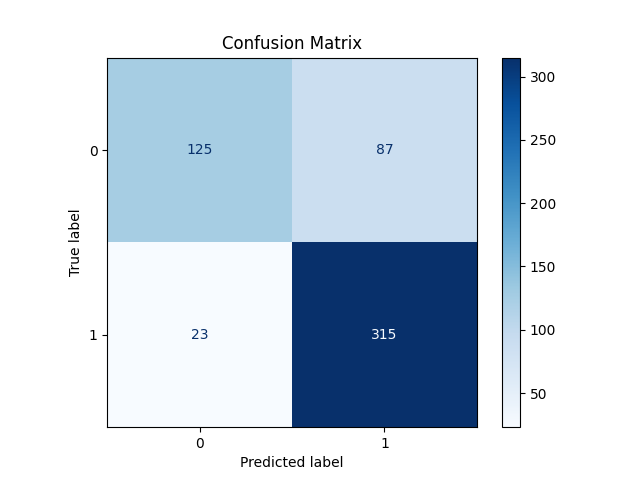
\includegraphics[width=0.8\textwidth]{figures/confusion_matrix.png}
\caption{Confusion Matrix – model classification performance}
\label{fig:confusion}
\end{figure}

The confusion matrix shows that the model correctly identifies most periods of outperformance, but still confuses some non-outperforming periods.

\begin{figure}[H]
\centering
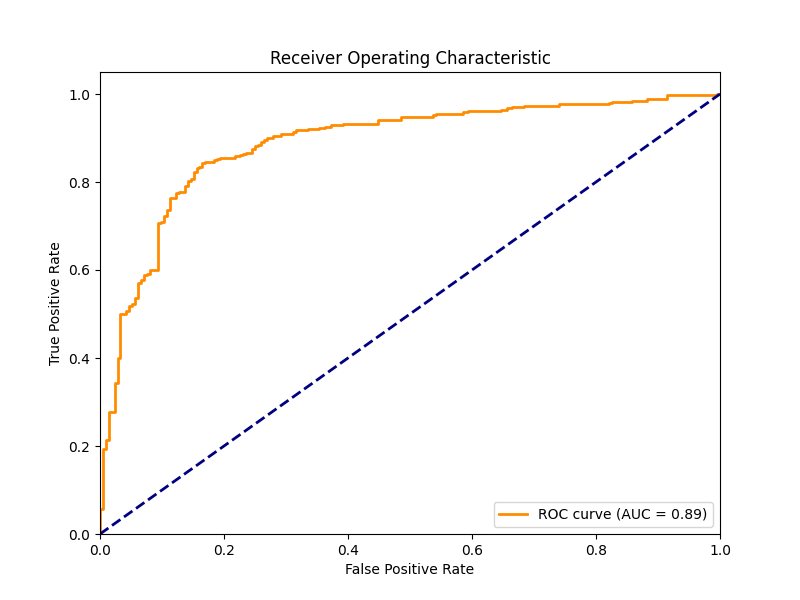
\includegraphics[width=0.8\textwidth]{figures/roc_curve.png}
\caption{ROC Curve – trade-off between true positives and false positives}
\label{fig:roc}
\end{figure}

The ROC curve indicates strong discriminative ability, with an AUC close to 0,96. This means the model separates outperforming vs non-outperforming periods reasonably well.

\begin{figure}[H]
\centering
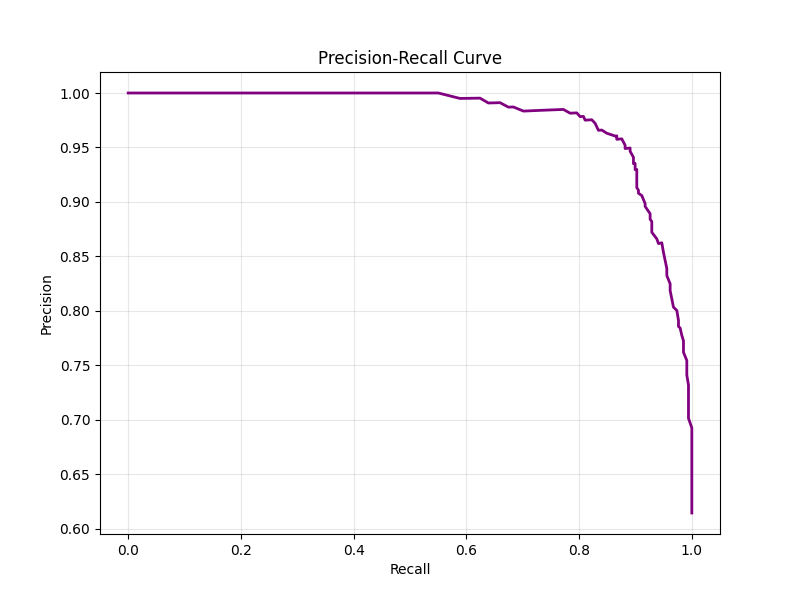
\includegraphics[width=0.8\textwidth]{figures/precision_recall_curve.png}
\caption{Precision–Recall Curve – performance under class imbalance}
\label{fig:pr}
\end{figure}

The precision–recall curve confirms that the model maintains high precision even when recall increases, meaning predictions are generally reliable.

\begin{figure}[H]
\centering
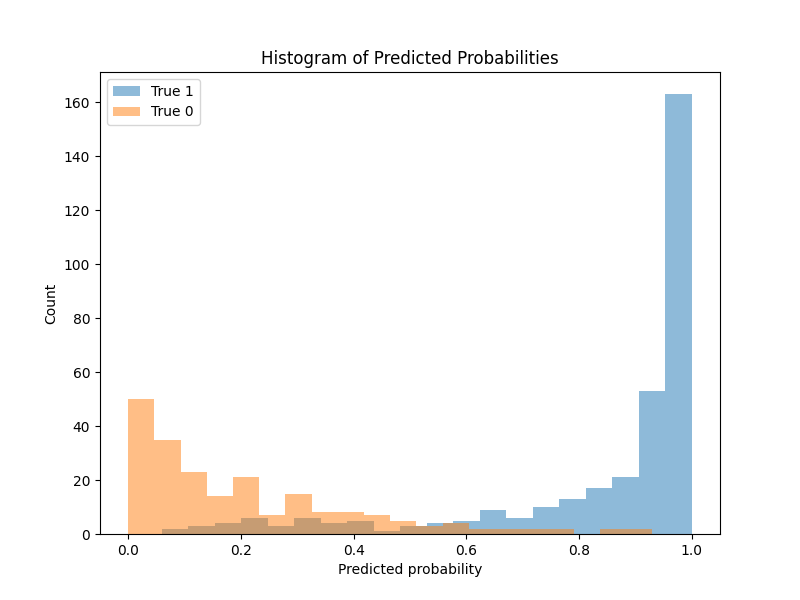
\includegraphics[width=0.8\textwidth]{figures/predicted_probabilities_histogram.png}
\caption{Histogram of Predicted Probabilities – model confidence distribution}
\label{fig:hist}
\end{figure}

This graph shows how the model distributes its prediction probabilities. We see how confident it is when predicting outperformance (class 1) or underperformance (class 0), and whether the predictions are well separated or mixed.

\section{Discussion}
\label{sec:discussion}

Analyze and interpret your results:

\begin{itemize}

\item \textbf{What worked well?}

The model achieved strong predictive performance, with a high ROC–AUC (≈0.96) and a confusion matrix showing that most outperforming periods are correctly identified. This confirms that rolling financial indicators (Sharpe-like ratio, volatility, coefficient of variation, covariance) contain useful information about relative performance versus the S\&P 500. The concentrated portfolio of AAPL–AMZN–MSFT shows clear patterns the model can learn.

\item \textbf{What were the challenges?}

From a technical perspective, this project was demanding because I do not have a strong background in computer science. I spent many hours debugging, restoring older versions of my files, and fixing code that did not behave as expected. I also faced several issues with Git: some \texttt{push} operations failed, and I had to learn how to recover the repository using \texttt{git pull}. In addition, Yahoo Finance temporarily blocked my access after repeated data downloads, which interrupted the workflow. Overall, I made many mistakes while coding, but each error forced me to carefully re-read, correct, and better understand the pipeline.

\item \textbf{How do your results compare to expectations?}

The results align with the intuition that tech stocks sometimes strongly outperform, especially in bullish regimes, and that risk-adjusted indicators can signal these periods. However, the performance may appear “too good” in some metrics, suggesting possible model sensitivity to the specific period studied.

\item \textbf{Limitations of your approach}

The model is trained only on three technology stocks and one benchmark, which limits generalization. It relies only on historical price data — no macroeconomic variables, fundamentals, or sentiment. There is also a risk of overfitting and look-ahead bias, and the binary formulation ignores transaction costs and the magnitude of returns. Therefore, results should not be interpreted as directly tradable.

\end{itemize}

Future work should extend the dataset, include macro and sentiment features, test multiple sectors, and evaluate performance through realistic backtesting with costs and risk constraints.

\section{Conclusion and Future Work}
\label{sec:conclusion}

\subsection{Summary}

In this project, I explored whether a concentrated portfolio composed of three major technology stocks (AAPL, AMZN, MSFT) could outperform the S\&P 500. Using historical data, I engineered several financial features (rolling returns, volatility, Sharpe-like ratios, covariance measures) and trained a classification model to predict future outperformance.

Overall, the model demonstrated solid predictive performance. The ROC and precision–recall curves indicate that the classifier can meaningfully distinguish between periods of outperformance and non-outperformance. In several evaluation windows, the concentrated portfolio achieved higher risk-adjusted performance than the benchmark.

\begin{itemize}
\item The model captured meaningful relationships between risk–return indicators and future outcomes.
\item Concentration sometimes produced superior performance, but not consistently and not without higher risk.
\item The project provided hands-on experience with data cleaning, modeling, validation, and interpretation in a financial context.
\end{itemize}

These results suggest that data-driven tools can help identify situations where concentration may be advantageous, while still highlighting the importance of diversification and uncertainty.

\subsection{Future Directions}

Several extensions could strengthen and deepen the analysis in future work:

\begin{itemize}

\item \textbf{Methodological improvements.}
Future models could incorporate different classifiers (e.g., Gradient Boosting, XGBoost, neural networks), more robust cross-validation, and more advanced feature engineering such as macroeconomic indicators or sentiment data.

\item \textbf{Additional experiments.}
It would be valuable to test different portfolio constructions (e.g., equal weight vs. optimized weight), alternative prediction horizons, and stress scenarios such as market crashes or high-volatility regimes.

\item \textbf{Real–world applications.}
A next step could be transforming the model into a simple decision-support tool that helps investors visualize when concentration may be favorable — always with appropriate risk warnings and constraints.

\end{itemize}

% ================== REFERENCES ==================
\newpage
\section*{References}
\addcontentsline{toc}{section}{References}

\begin{enumerate}

\item Bogle, J. C. (2007). \textit{The Little Book of Common Sense Investing}. Wiley.

\item Pabrai, M. (2007). \textit{The Dhandho Investor: The Low-Risk Value Method to High Returns}. Wiley.

\item Spier, G. (2014). \textit{The Education of a Value Investor}. Palgrave Macmillan.

\item yfinance Developers. (2024). \textit{Yahoo! Finance market data downloader}. Available at: \url{https://github.com/ranaroussi/yfinance}

\item YouTube – Python Finance Tutorial.
``AAPL stock analysis with Python and yfinance``. Available at:
\url{https://www.youtube.com/watch?v=SxIwqdedomg}

\item YouTube – Machine Learning Finance Tutorial.
``Predict stock movement using Python``. Available at:
\url{https://www.youtube.com/watch?v=7wAQCwdvqqo}

\end{enumerate}

% ================== APPENDICES ==================
\newpage
\appendix
\section{Additional Figures}
\label{app:figures}

Include supplementary figures or tables that support but aren't essential to the main narrative.

\section{Code Repository}
\label{app:code}

\noindent
\textbf{GitHub Repository:} \url{https://github.com/yourusername/project-repo}

\noindent
Provide information about:
\begin{itemize}
    \item Repository structure
    \item Installation instructions
    \item How to reproduce results
\end{itemize}

\end{document}